\documentclass[tikz,crop]{standalone}

\begin{document}
% Created by tikzDevice version 0.12.3.1 on 2022-01-17 17:24:13
% !TEX encoding = UTF-8 Unicode
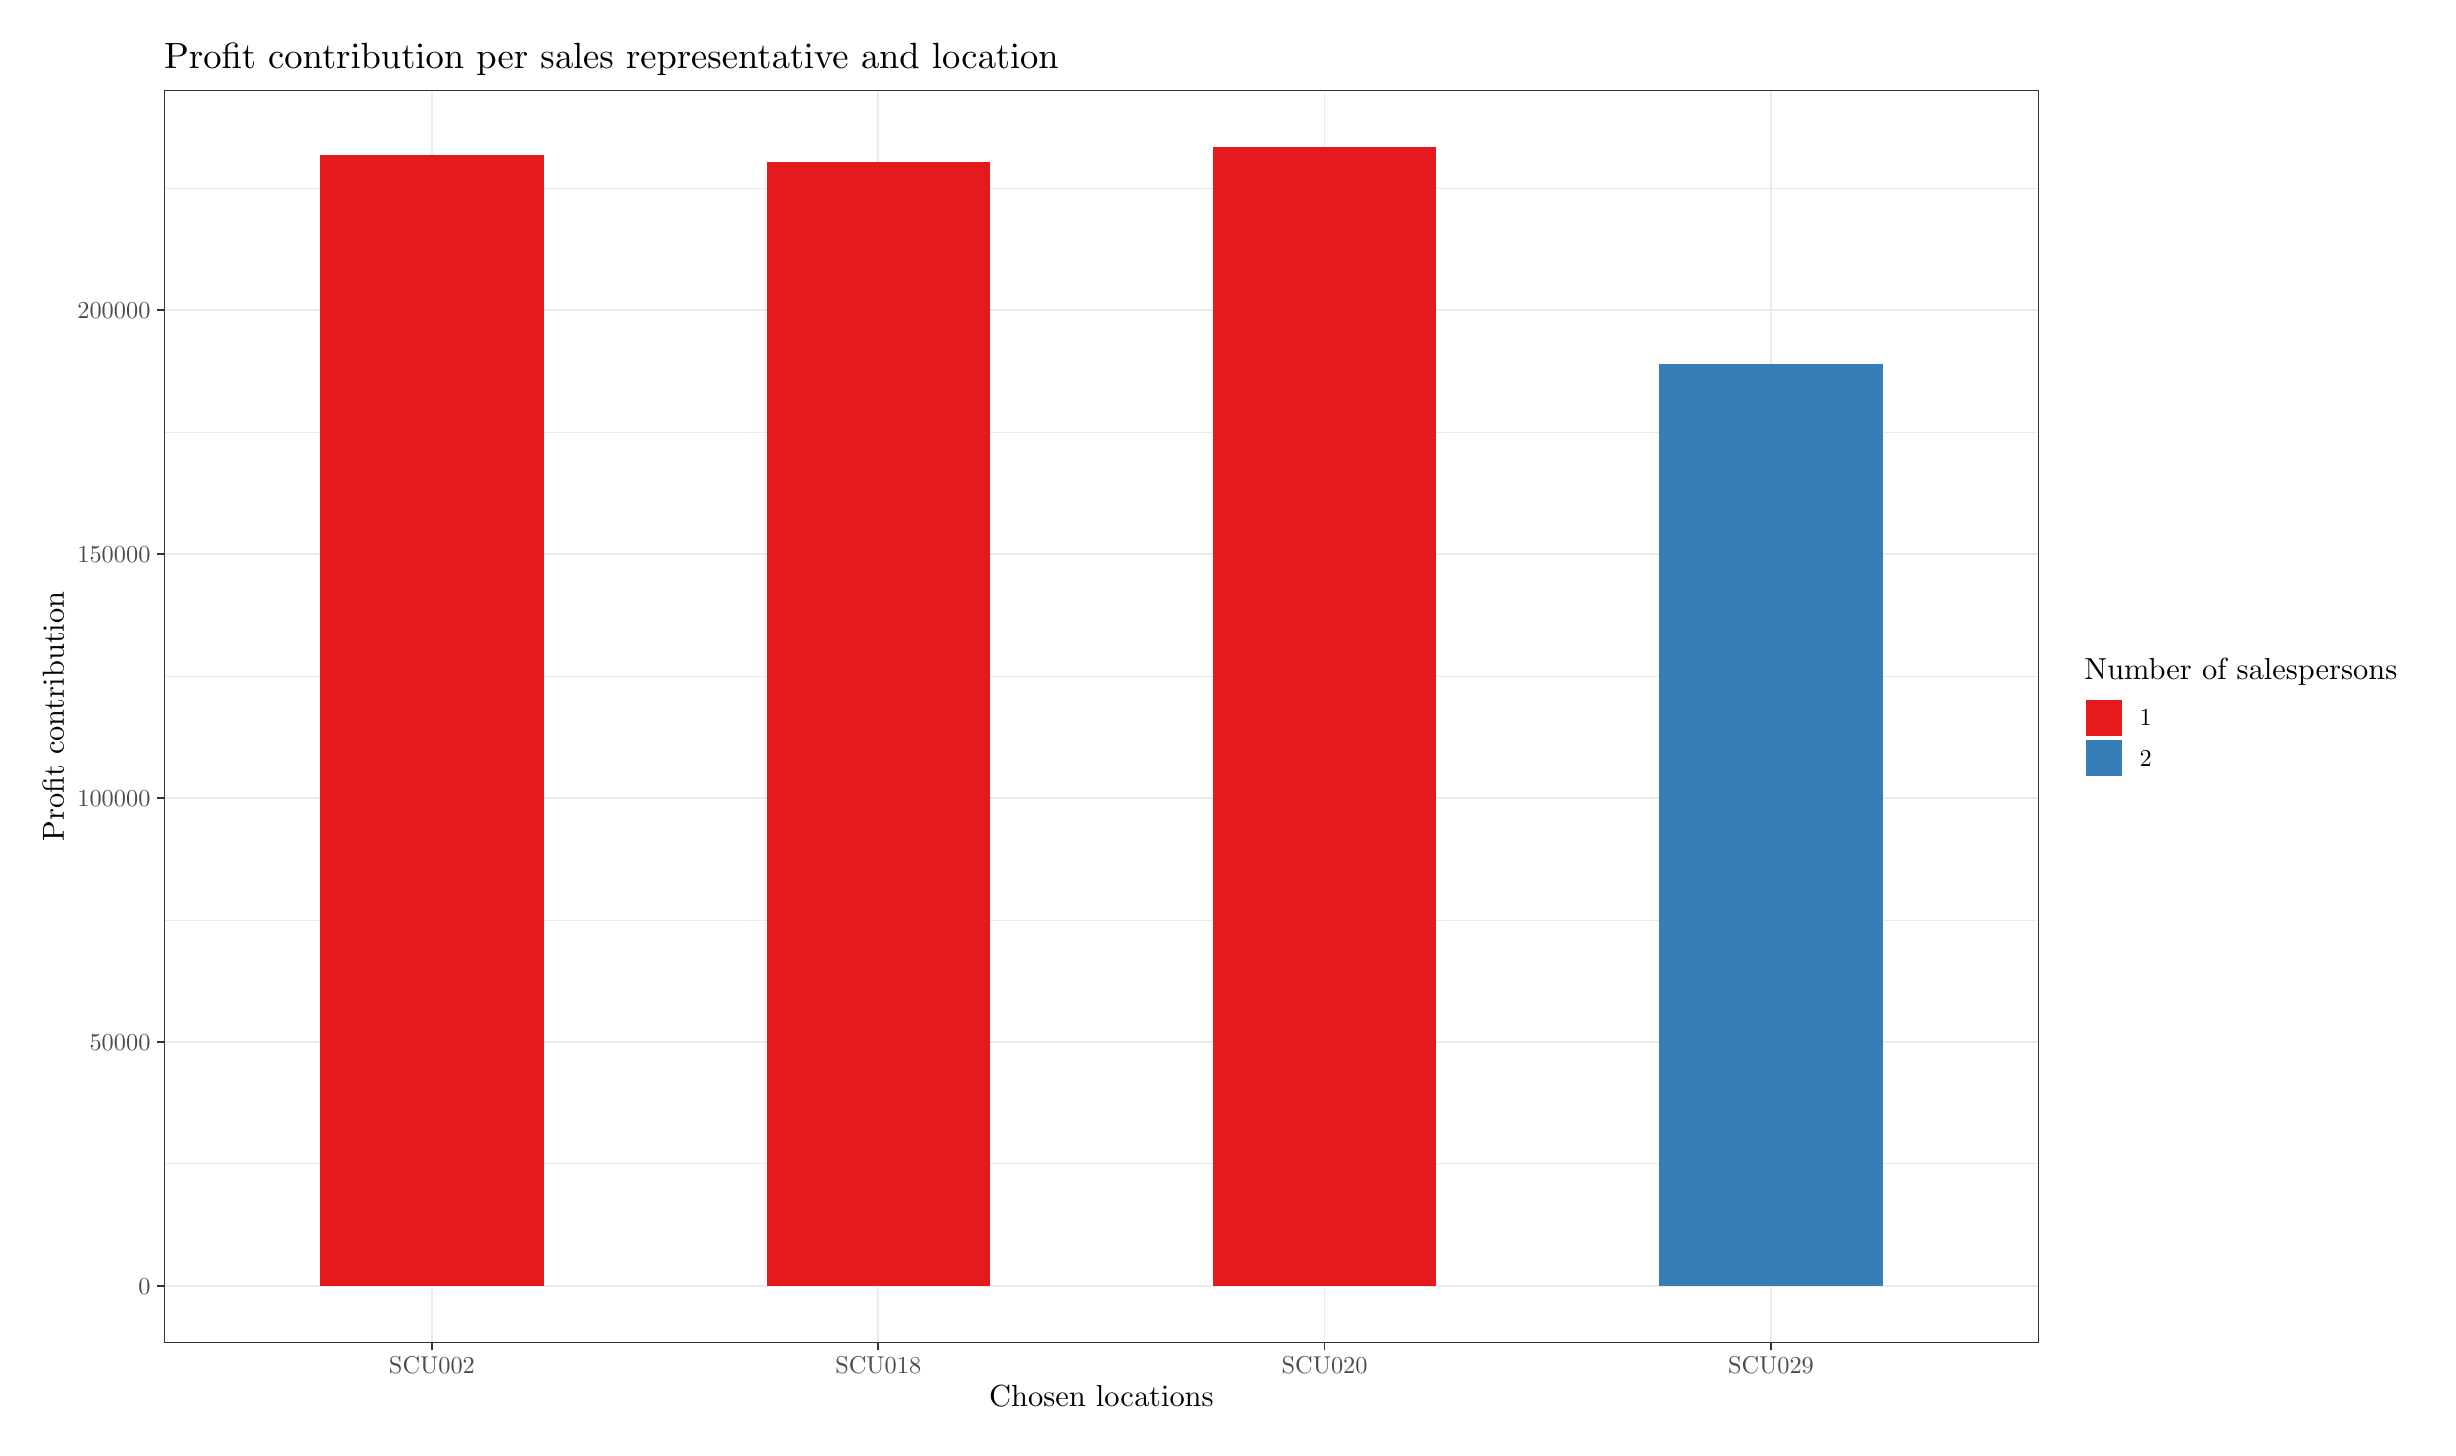
\begin{tikzpicture}[x=1pt,y=1pt]
\definecolor{fillColor}{RGB}{255,255,255}
\path[use as bounding box,fill=fillColor,fill opacity=0.00] (0,0) rectangle (867.24,505.89);
\begin{scope}
\path[clip] (  0.00,  0.00) rectangle (867.24,505.89);
\definecolor{drawColor}{RGB}{255,255,255}
\definecolor{fillColor}{RGB}{255,255,255}

\path[draw=drawColor,line width= 0.6pt,line join=round,line cap=round,fill=fillColor] (  0.00,  0.00) rectangle (867.24,505.89);
\end{scope}
\begin{scope}
\path[clip] ( 49.31, 30.69) rectangle (726.71,483.23);
\definecolor{fillColor}{RGB}{255,255,255}

\path[fill=fillColor] ( 49.31, 30.69) rectangle (726.71,483.23);
\definecolor{drawColor}{gray}{0.92}

\path[draw=drawColor,line width= 0.3pt,line join=round] ( 49.31, 95.33) --
	(726.71, 95.33);

\path[draw=drawColor,line width= 0.3pt,line join=round] ( 49.31,183.47) --
	(726.71,183.47);

\path[draw=drawColor,line width= 0.3pt,line join=round] ( 49.31,271.61) --
	(726.71,271.61);

\path[draw=drawColor,line width= 0.3pt,line join=round] ( 49.31,359.76) --
	(726.71,359.76);

\path[draw=drawColor,line width= 0.3pt,line join=round] ( 49.31,447.90) --
	(726.71,447.90);

\path[draw=drawColor,line width= 0.6pt,line join=round] ( 49.31, 51.26) --
	(726.71, 51.26);

\path[draw=drawColor,line width= 0.6pt,line join=round] ( 49.31,139.40) --
	(726.71,139.40);

\path[draw=drawColor,line width= 0.6pt,line join=round] ( 49.31,227.54) --
	(726.71,227.54);

\path[draw=drawColor,line width= 0.6pt,line join=round] ( 49.31,315.69) --
	(726.71,315.69);

\path[draw=drawColor,line width= 0.6pt,line join=round] ( 49.31,403.83) --
	(726.71,403.83);

\path[draw=drawColor,line width= 0.6pt,line join=round] (146.08, 30.69) --
	(146.08,483.23);

\path[draw=drawColor,line width= 0.6pt,line join=round] (307.37, 30.69) --
	(307.37,483.23);

\path[draw=drawColor,line width= 0.6pt,line join=round] (468.65, 30.69) --
	(468.65,483.23);

\path[draw=drawColor,line width= 0.6pt,line join=round] (629.94, 30.69) --
	(629.94,483.23);
\definecolor{fillColor}{RGB}{228,26,28}

\path[fill=fillColor] (105.76, 51.26) rectangle (186.40,459.99);

\path[fill=fillColor] (267.04, 51.26) rectangle (347.69,457.22);

\path[fill=fillColor] (428.33, 51.26) rectangle (508.97,462.66);
\definecolor{fillColor}{RGB}{55,126,184}

\path[fill=fillColor] (589.62, 51.26) rectangle (670.26,384.20);
\definecolor{drawColor}{gray}{0.20}

\path[draw=drawColor,line width= 0.6pt,line join=round,line cap=round] ( 49.31, 30.69) rectangle (726.71,483.23);
\end{scope}
\begin{scope}
\path[clip] (  0.00,  0.00) rectangle (867.24,505.89);
\definecolor{drawColor}{gray}{0.30}

\node[text=drawColor,anchor=base east,inner sep=0pt, outer sep=0pt, scale=  0.88] at ( 44.36, 48.23) {0};

\node[text=drawColor,anchor=base east,inner sep=0pt, outer sep=0pt, scale=  0.88] at ( 44.36,136.37) {50000};

\node[text=drawColor,anchor=base east,inner sep=0pt, outer sep=0pt, scale=  0.88] at ( 44.36,224.51) {100000};

\node[text=drawColor,anchor=base east,inner sep=0pt, outer sep=0pt, scale=  0.88] at ( 44.36,312.66) {150000};

\node[text=drawColor,anchor=base east,inner sep=0pt, outer sep=0pt, scale=  0.88] at ( 44.36,400.80) {200000};
\end{scope}
\begin{scope}
\path[clip] (  0.00,  0.00) rectangle (867.24,505.89);
\definecolor{drawColor}{gray}{0.20}

\path[draw=drawColor,line width= 0.6pt,line join=round] ( 46.56, 51.26) --
	( 49.31, 51.26);

\path[draw=drawColor,line width= 0.6pt,line join=round] ( 46.56,139.40) --
	( 49.31,139.40);

\path[draw=drawColor,line width= 0.6pt,line join=round] ( 46.56,227.54) --
	( 49.31,227.54);

\path[draw=drawColor,line width= 0.6pt,line join=round] ( 46.56,315.69) --
	( 49.31,315.69);

\path[draw=drawColor,line width= 0.6pt,line join=round] ( 46.56,403.83) --
	( 49.31,403.83);
\end{scope}
\begin{scope}
\path[clip] (  0.00,  0.00) rectangle (867.24,505.89);
\definecolor{drawColor}{gray}{0.20}

\path[draw=drawColor,line width= 0.6pt,line join=round] (146.08, 27.94) --
	(146.08, 30.69);

\path[draw=drawColor,line width= 0.6pt,line join=round] (307.37, 27.94) --
	(307.37, 30.69);

\path[draw=drawColor,line width= 0.6pt,line join=round] (468.65, 27.94) --
	(468.65, 30.69);

\path[draw=drawColor,line width= 0.6pt,line join=round] (629.94, 27.94) --
	(629.94, 30.69);
\end{scope}
\begin{scope}
\path[clip] (  0.00,  0.00) rectangle (867.24,505.89);
\definecolor{drawColor}{gray}{0.30}

\node[text=drawColor,anchor=base,inner sep=0pt, outer sep=0pt, scale=  0.88] at (146.08, 19.68) {SCU002};

\node[text=drawColor,anchor=base,inner sep=0pt, outer sep=0pt, scale=  0.88] at (307.37, 19.68) {SCU018};

\node[text=drawColor,anchor=base,inner sep=0pt, outer sep=0pt, scale=  0.88] at (468.65, 19.68) {SCU020};

\node[text=drawColor,anchor=base,inner sep=0pt, outer sep=0pt, scale=  0.88] at (629.94, 19.68) {SCU029};
\end{scope}
\begin{scope}
\path[clip] (  0.00,  0.00) rectangle (867.24,505.89);
\definecolor{drawColor}{RGB}{0,0,0}

\node[text=drawColor,anchor=base,inner sep=0pt, outer sep=0pt, scale=  1.10] at (388.01,  7.64) {Chosen locations};
\end{scope}
\begin{scope}
\path[clip] (  0.00,  0.00) rectangle (867.24,505.89);
\definecolor{drawColor}{RGB}{0,0,0}

\node[text=drawColor,rotate= 90.00,anchor=base,inner sep=0pt, outer sep=0pt, scale=  1.10] at ( 13.08,256.96) {Profit contribution};
\end{scope}
\begin{scope}
\path[clip] (  0.00,  0.00) rectangle (867.24,505.89);
\definecolor{fillColor}{RGB}{255,255,255}

\path[fill=fillColor] (737.71,229.40) rectangle (861.74,284.52);
\end{scope}
\begin{scope}
\path[clip] (  0.00,  0.00) rectangle (867.24,505.89);
\definecolor{drawColor}{RGB}{0,0,0}

\node[text=drawColor,anchor=base west,inner sep=0pt, outer sep=0pt, scale=  1.10] at (743.21,270.38) {Number of salespersons};
\end{scope}
\begin{scope}
\path[clip] (  0.00,  0.00) rectangle (867.24,505.89);
\definecolor{fillColor}{RGB}{255,255,255}

\path[fill=fillColor] (743.21,249.35) rectangle (757.67,263.81);
\end{scope}
\begin{scope}
\path[clip] (  0.00,  0.00) rectangle (867.24,505.89);
\definecolor{fillColor}{RGB}{228,26,28}

\path[fill=fillColor] (743.92,250.06) rectangle (756.95,263.09);
\end{scope}
\begin{scope}
\path[clip] (  0.00,  0.00) rectangle (867.24,505.89);
\definecolor{fillColor}{RGB}{255,255,255}

\path[fill=fillColor] (743.21,234.90) rectangle (757.67,249.35);
\end{scope}
\begin{scope}
\path[clip] (  0.00,  0.00) rectangle (867.24,505.89);
\definecolor{fillColor}{RGB}{55,126,184}

\path[fill=fillColor] (743.92,235.61) rectangle (756.95,248.64);
\end{scope}
\begin{scope}
\path[clip] (  0.00,  0.00) rectangle (867.24,505.89);
\definecolor{drawColor}{RGB}{0,0,0}

\node[text=drawColor,anchor=base west,inner sep=0pt, outer sep=0pt, scale=  0.88] at (763.17,253.55) {1};
\end{scope}
\begin{scope}
\path[clip] (  0.00,  0.00) rectangle (867.24,505.89);
\definecolor{drawColor}{RGB}{0,0,0}

\node[text=drawColor,anchor=base west,inner sep=0pt, outer sep=0pt, scale=  0.88] at (763.17,239.09) {2};
\end{scope}
\begin{scope}
\path[clip] (  0.00,  0.00) rectangle (867.24,505.89);
\definecolor{drawColor}{RGB}{0,0,0}

\node[text=drawColor,anchor=base west,inner sep=0pt, outer sep=0pt, scale=  1.32] at ( 49.31,491.30) {Profit contribution per sales representative and location};
\end{scope}
\end{tikzpicture}

\end{document}